\documentclass{article}

\usepackage[latin1]{inputenc}
\usepackage{pgfplots}
\usepackage{tikz}

\pgfplotsset{compat=1.10}

% GNUPLOT required
\begin{document}
\pagestyle{empty}

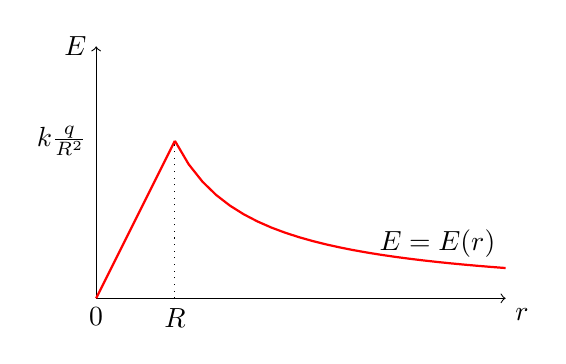
\begin{tikzpicture}
	\draw[->] (0,0) -- (5.2,0) node[below right] {$r$};
	\draw[->] (0,0) -- (0,3.2) node[left] {$E$};
	\node[below] (0, 0) {$0$};
	\draw[black] (0, 0) -- (0, 2) node[left] {$k\frac{q}{R^2}$};
	\draw[black] (0, 0) -- (1, 0) node[below] {$R$};
	\draw[black, thin, dotted] (1, 0) -- (1, 2);

	\draw[red, thick, domain=0:1] plot (\x, {2*\x});
    \draw[red, thick, domain=1:5.2] plot (\x, {2/\x}) node[black, above left] {$E=E(r)$};
\end{tikzpicture}


\end{document}